\subsection{Kryptografische Inferenz}\label{sec:krypto_inferenz}

Wird ein Modell auf einen fremden Server (beispielsweise in einer Cloud) deployt, wäre es möglich, dass der Provider des Servers Informationen über die Daten, die zur Vorhersage genutzt werden, herausfindet.
Dies wird sowohl durch Homomorphe Verschlüsselung als auch durch Funktionale Verschlüsselung verhindert.
Beide Methoden sorgen dafür, dass Daten verschlüsselt in das Modell gegeben werden, sodass sich diese Daten zu keinem Zeitpunkt unverschlüsselt auf dem fremden Server befinden.
Auch andere Methoden, wie Garbled Circuits, erlauben die Inferenz des Modells, ohne dass die Daten zu einem Zeitpunkt unverschlüsselt veröffentlicht werden.


\subsubsection*{Inferenz mittels Homomorpher Verschlüsselung}
Das bereits in Kapitel \ref{sec:homomorphe_verschlüsselung} und \ref{sec:verteiltes_lernen} beschrieben Framework von Takabi et al. \cite{P-104}, zeigt, wie Homomorphe Verschlüsselung genutzt werden kann, um die Inferenz des Modells durchzuführen.
Dabei wird ein eingeschränkt homomorphes Verschlüsselungssystem genutzt, um die Daten eines Nutzers verschlüsselt durch das Modell zu interferieren.
Wird das Rauschen des Verschlüsselungssystems zu groß (festgelegter Schwellenwert), erhält der Nutzer den aktuellen Zustand, muss diesen entschlüsseln und neu verschlüsseln, bevor die Berechnung des Modells fortgesetzt werden kann.

Eine weitere Möglichkeit Homomorphe Verschlüsselung für die Inferenz eines Modells zu nutzen, wird von Gilad-Bachrach et al. mit dem Framework CryptoNets \cite{P-54} vorgestellt.
Die Architektur des Modells ist jedoch eingeschränkt. 
Als Aktivierungsfunktion wird eine Quadratfunktion angewendet (anstelle von beispielsweise ReLU) und als Pooling Operation wird ein Durchschnitts-Pooling genutzt.
Um die Performance zu steigern, können Schichten des Netzes miteinander verbunden werden. 
Dies ist bei benachbarten Schichten aus linearen Funktionen (in der Regel Schichten zwischen Aktivierungsfunktionen) möglich.
Zusätzlich kann bei einer Klassifikation auch die letzte Schicht weggelassen werden, da einfach der höchste Wert der Klasse entspricht. 
Dadurch können keine Wahrscheinlichkeiten der Vorhersagen mitgegeben werden, die vorhergesagte Klasse bleibt dennoch gleich.
CryptoNets nutzt eine eingeschränkt homomorphe Verschlüsselung, welche auf Gittern und algebraischen Ringen basiert. 
Die Anzahl an Berechnungen ist dabei an die Struktur und Tiefe des Neuronalen Netzes gebunden.
Abhängig von der Größe der Sicherheitsparameter werden tiefere Neuronale Netze unterstützt.
Die Autoren demonstrieren CryptoNets anhand eines Neuronalen Netzes, welche eine Klassifikation des MNIST Datensatzes \cite{D-MNIST} vornimmt.
Das Neuronale Netz ist besitzt dabei zwei Faltungsschichten (Convolutional Layer), die jeweils von einer Aktivierungsfunktion und Pooling Layer erweitert werden.
Zusätzlich werden zwei vollständig verbundene Schichten (Filly Connected Layer) hinzugefügt, wobei eine davon auch als Output Schicht dient.
Mit einer Batch Size von 4096 Bildern ($28 \times 28$ Pixel), benötigt die Inferenz des Modells (auf einer Server-CPU aus dem Jahr 2012) 250 Sekunden. 
Dies würde, bei voller Auslastung, fast 60.000 Vorhersagen pro Stunde entsprechen.
Die Ver- und Entschlüsselung benötigen knapp 50 Sekunden zusätzlich, würde aber in einer Client-Server Architektur vom Client übernommen werden.
Zusätzlich würden in der Client-Server Architektur pro Batch 370 Megabyte an Daten übertragen werden.

Chabanne et al. \cite{P-55} verbesserten den Ansatz von CryptoNets, indem zusätzlich Fokus auf die Güte des Modells gelegt wird. 
Komplexere Modelle, die bei vielen Aufgaben eine verbesserte Performance aufweisen, sind nicht für CryptoNets geeignet.
Dies liegt daran, dass komplexere Modelle mehr Aktivierungsfunktionen enthalten. 
Werden dafür Quadratfunktionen genutzt, könnte das Training instabil werden, da der Gradient dieser Funktionen beliebig groß werden könnte.
Der Ansatz nutzt anstelle von Quadratfunktionen demnach wieder die ReLU Funktion als Aktivierungsfunktion während des Trainings.
Bei der Inferenz des Modells auf verschlüsselten Daten, wird die ReLU Funktion mittels einer Polynomfunktion approximiert.
Diese Polynomfunktion wird im Voraus mittels Regression ermittelt. 
Der Grad der Polynomfunktion kann dabei die Genauigkeit der Approximation und auch die benötigte Rechenleistung beeinflussen.
Der Grad 4 der Polynomfunktion zeigte bei der Evaluierung eine ausreichend gute Approximation, sodass Modelle verschlüsselt eine fast genauso gute Güte haben wie unverschlüsselt.
Ein Neuronales Netz mit 9 Schichten (eine davon ReLU) für den MNIST Datensatz \cite{D-MNIST}, welches unverschlüsselt eine Genauigkeit von 97,95\% hat, würde mit dem Ansatz eine Genauigkeit von 97,84\% erreichen.
Bei tieferen Neuronalen Netzen fällt die Differenz größer aus. 
Bei einem Netz mit 24 Schichten (sechs davon ReLU), fällt die Genauigkeit von 99.59\% auf 97.91\%.
Der Ansatz von Chabanne et al. \cite{P-55} würde demnach das Training im Vergleich zu CryptoNets \cite{P-54} stabilisieren, jedoch würde durch die Approximation Genauigkeit einbüßt werden.


\subsubsection*{Inferenz mittels Funktionaler Verschlüsselung}
Das CryptoNN Framework \cite{P-53}, welches in Kapitel \ref{sec:funktionale_verschlüsselung} beschrieben wurde, enthält bereits einen den Feedforward Schritt eines Neuronalen Netzes mit Funktionaler Verschlüsselung, welcher der Inferenz des Modells entspricht.
Dabei wird nur die erste Schicht des Netzes verschlüsselt berechnet, die restliche Berechnung erfolgt unverschlüsselt.

Dufour-Sans el at. \cite{P-105} stellen eine alternative Möglichkeit vor, Funktionale Verschlüsselung für Neuronale Netze zu nutzen.
Im Vergleich zu CryptoNN, kann die Inferenz des Modells bei diesem Ansatz ganz vorgenommen werden.
Dabei wird eine effiziente Funktionale Verschlüsselung genutzt, die jedoch nur Polynome des Grades 2 berechnen kann.
Folglich werden nicht alle Operationen unterstützt, sondern nur lineare Schichten, Convolutions mit einem Durchschnitts-Pooling und Aktivierungsfunktionen, die sich mit Polynomen approximieren lassen.
Anstelle einer Aktivierungsfunktion an der Output Schicht, wird der größte Wert als Vorhersage genutzt.
Mit dieser Methode konnten die Autoren ein Modell trainieren, welches 97,54\% Genauigkeit auf dem MNIST Datensatz \cite{D-MNIST} erreicht und die Inferenz eines Datensatzes auf einer CPU in knapp 13 Sekunden durchführt.
Das Paper wurde in einer umfassenderen Version von Ryffel et al. \cite{P-46} veröffentlicht.
Dieses enthält den Vorschlag, nur die ersten Schichten des Modells mit Funktionaler Verschlüsselung zu berechnen. 
Der Vorteil dieser Variante ist es, dass die unverschlüsselten Schichten mehr Operationen unterstützen und dadurch die Güte des Modells verbessern kann.

\subsubsection*{Inferenz durch Secure Multi-Party Computation}
DeepSecure \cite{P-71}, welches in Kapitel \ref{sec:verteiltes_lernen} beschrieben wurde, enthält bereits einen Möglichkeit, den Output des Modells mittels Yao's Garbled Circuits zu berechnen.
Dabei wird das Modell als ein Boolescher Schaltkreis aus XOR und XNOR Gattern mit zwei Eingabegattern dargestellt, welches anschließend gemeinsam von Nutzer und Server ausgewertet werden.

Ein weiteres Framework zur Evaluation eines Neuronalen Netzes mittels Secure Multi-Party Computation wurde von Riazi et al. \cite{P-72} mit dem Namen Chameleon vorgestellt.
Dieses nutzt neben Yao's Garbled Circuits noch zwei weitere Methoden: das Goldreich-Micali-Wigderson (GMW) Protokoll und Secret Sharing, zu Deutsch Geheimnisteilung.
Das GMW Protokoll ist eine Alternative zu Yao's Garbled Circuits, bei dem ebenfalls zwei Parteien gemeinsam, ohne Teilen der privaten Daten, eine Berechnung durchführen können.
Ebenfalls wird die Berechnung als Boolescher Schaltkreis dargestellt, welcher aus XOR und AND Gattern besteht. 
Da die XOR Operation assoziativ ist, können diese Operationen im Vorraus in einer sogenannten Offline Phase zusammengefasst werden. 
Lediglich die AND Gatter benötigen eine Kommunikation der beiden Parteien, was zusätzlich auch rechenintensiver ist.
Demnach ist die Anzahl der AND Gatter entscheidend für die Performance.
Gibt es wenige, so kann die Performance des GMW Protokolls besser sein, als Yao's Garbled Circuits.
Bei dem sogenannten Secret Sharing wird ein Geheimnis unter mehreren Parteien aufgeteilt, sodass nur die Kombination aller Teile das korrekte Geheimnis rekonstruierbar macht.
Keiner der Parteien kann demnach ohne die anderen Parteien das Geheimnis wiederherstellen. 
Chameleon nutzt Additives Secret Sharing, was bedeutet, die einzelnen Teile müssen addiert werden, um den ursprünglichen Wert zu erhalten.
Zusätzlich findet das Secret Sharing auf einem algebraischen Ring $\mathbb{Z}$ mod $2^{k} $ statt, was dazu führt, dass Rechenoperationen mit bekannten Konstanten, ohne Kommunikation, auf einzelnen Teilen des Geheimnisses durchgeführt werden kann.

\begin{figure}[!htb]
    \centering
    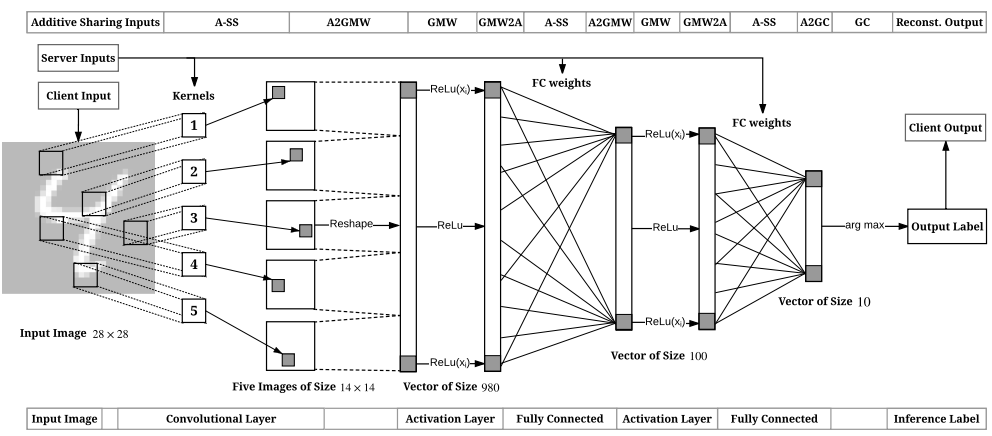
\includegraphics[width=15cm]{figures/chameleon.png}
    \caption{Chameleon Framework \cite{P-72}}
    \label{fig:chameleon}
\end{figure} 

Das Chameleon Framework kombiniert diese Methoden, um eine effiziente, kryptografisch sichere Inferenz für Neuronale Netze zu ermöglichen. Abbildung \ref{fig:chameleon} zeigt, wie das Framework an einem Modell des MNIST Datensatzes \cite{D-MNIST} angewendet wird.
Convolution Layer und Fully Connected Layer werden dabei mittels Additive Secret Sharing und dem GMW Protokoll berechnet.
Die Klasse des Datenpunktes wird dabei durch den höchsten Wert der letzten Sicht wird mittels Yao's Garbled Circuits extrahiert.
Das dargestellte Modell benötigt knapp 2,5 Sekunden für eine Inferenz, welche eine Batch Größe von 8196 Bildern unterstützt.
Damit wären, auf einer Server-CPU, über 11 Millionen Vorhersagen pro Stunde möglich.
Dabei bleibt die Genauigkeit des Modells im Vergleich zur unverschlüsselten Inferenz gleich.

Neben den bereits beschriebenen Lösungen gibt es eine Reihe weiterer Frameworks zur kryptografischen Inferenz eines Modells. 
Diese setzen sich alle den bereits beschriebenen Methoden zusammen, aber kombinieren oder optimieren diese an einigen Stellen.
So verknüpft das MiniONN Framework \cite{P-59} die Techniken Oblivious Transfer, Yao's Garbled Circuits und Secret Sharing. 
Optional können einige Schritte mit Homomorpher Verschlüsselung angepasst werden, was die Last von Kommunikation auf Rechenleistung verlegt.
XONN \cite{P-106} zeigt, wie der Boolesche Schaltkreis eines Neuronalen Netzes transformiert werden kann, sodass weniger Rechenintensive Gatter vorkommen.
